\documentclass[main.tex]{subfiles}
\begin{document}

\section{Acceptors and Transducers}
\label{sec:acceptors_transducers}

\subsection{Automata}
\label{sec:automata}

The broad class of graphs we are going to look at are finite-state automata.
These include deterministic finite-state automata (DFAs) and non-deterministic
finite-state automata (NFAs). More specifically we will consider a
generalization of DFAs and NFAs called weighted finite-state acceptors (WFSAs).
That's a mouthful, so I will just call them \emph{acceptors}. We will also consider
a further generalization of an acceptor called a \emph{transducer} (weighted
finite-state transducers or WFSTs). The following figure shows the relation
between these three graphs; transducers, acceptors, and automtata. Transducers
are the most expressive in terms of their representational power, followed by
acceptors followed by unweighted automata.

\begin{figure}
    \centering
    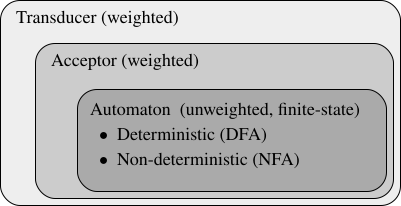
\includegraphics[width=0.5]{wfsa_classes}
    \caption{A hierarchy of automata classes from general to specific in terms
    of representation power. Weighted transducers can represent anything that
    weighted acceptors can represent. Weighted acceptors in turn can represent
    any unweighted finite-state automata.}
    \label{fig:wfsa_classes}
\end{figure}

\end{document}
